% Created 2020-05-06 三 21:31
% Intended LaTeX compiler: pdflatex
\documentclass[11pt]{article}
\usepackage[utf8]{inputenc}
\usepackage[T1]{fontenc}
\usepackage{graphicx}
\usepackage{grffile}
\usepackage{longtable}
\usepackage{wrapfig}
\usepackage{rotating}
\usepackage[normalem]{ulem}
\usepackage{amsmath}
\usepackage{textcomp}
\usepackage{amssymb}
\usepackage{capt-of}
\usepackage{imakeidx}
\usepackage{hyperref}
\usepackage{minted}
\author{wugouzi}
\date{\today}
\title{}
\hypersetup{
 pdfauthor={wugouzi},
 pdftitle={},
 pdfkeywords={},
 pdfsubject={},
 pdfcreator={Emacs 26.3 (Org mode 9.3.6)}, 
 pdflang={English}}
\begin{document}

\tableofcontents \clearpage\% Created 2020-05-06 三 21:30
\% Intended \LaTeX{} compiler: pdflatex
\documentclass[11pt]{article}
\usepackage[utf8]{inputenc}
\usepackage[T1]{fontenc}
\usepackage{graphicx}
\usepackage{grffile}
\usepackage{longtable}
\usepackage{wrapfig}
\usepackage{rotating}
\usepackage[normalem]{ulem}
\usepackage{amsmath}
\usepackage{textcomp}
\usepackage{amssymb}
\usepackage{capt-of}
\usepackage{imakeidx}
\usepackage{hyperref}
\usepackage{minted}
% TIPS
% \substack{a\\b} for multiple lines text





% pdfplots will load xolor automatically without option
\usepackage[dvipsnames]{xcolor}

\usepackage{forest}
% two-line text in node by [two \\ lines]
% \begin{forest} qtree, [..] \end{forest}
\forestset{
  qtree/.style={
    baseline,
    for tree={
      parent anchor=south,
      child anchor=north,
      align=center,
      inner sep=1pt,
    }}}
%\usepackage{flexisym}
% load order of mathtools and mathabx, otherwise conflict overbrace

\usepackage{mathtools}
%\usepackage{fourier}
\usepackage{pgfplots}
\usepackage{amsthm}
\usepackage{amsmath}
%\usepackage{unicode-math}
%
\usepackage{commath}
%\usepackage{,  , }
\usepackage{amsfonts}
\usepackage{amssymb}
% importing symbols https://tex.stackexchange.com/questions/14386/importing-a-single-symbol-from-a-different-font
%mathabx change every symbol
% use instead stmaryrd
%\usepackage{mathabx}
\usepackage{stmaryrd}
\usepackage{empheq}
\usepackage{tikz}
\usepackage{tikz-cd}
%\usepackage[notextcomp]{stix}
\usetikzlibrary{arrows.meta}
\usepackage[most]{tcolorbox}
%\utilde
%\usepackage{../../latexpackage/undertilde/undertilde}
% left and right superscript and subscript
\usepackage{actuarialsymbol}
\usepackage{threeparttable}
\usepackage{scalerel,stackengine}
\usepackage{stackrel}
% \stackrel[a]{b}{c}
\usepackage{dsfont}
% text font
\usepackage{newpxtext}
%\usepackage{newpxmath}

%\newcounter{dummy} \numberwithin{dummy}{section}
\newtheorem{dummy}{dummy}[section]
\theoremstyle{definition}
\newtheorem{definition}[dummy]{Definition}
\newtheorem{corollary}[dummy]{Corollary}
\newtheorem{lemma}[dummy]{Lemma}
\newtheorem{proposition}[dummy]{Proposition}
\newtheorem{theorem}[dummy]{Theorem}
\theoremstyle{definition}
\newtheorem{example}[dummy]{Example}
\theoremstyle{remark}
\newtheorem*{remark}{Remark}


\newcommand\what[1]{\ThisStyle{%
    \setbox0=\hbox{$\SavedStyle#1$}%
    \stackengine{-1.0\ht0+.5pt}{$\SavedStyle#1$}{%
      \stretchto{\scaleto{\SavedStyle\mkern.15mu\char'136}{2.6\wd0}}{1.4\ht0}%
    }{O}{c}{F}{T}{S}%
  }
}

\newcommand\wtilde[1]{\ThisStyle{%
    \setbox0=\hbox{$\SavedStyle#1$}%
    \stackengine{-.1\LMpt}{$\SavedStyle#1$}{%
      \stretchto{\scaleto{\SavedStyle\mkern.2mu\AC}{.5150\wd0}}{.6\ht0}%
    }{O}{c}{F}{T}{S}%
  }
}

\newcommand\wbar[1]{\ThisStyle{%
    \setbox0=\hbox{$\SavedStyle#1$}%
    \stackengine{.5pt+\LMpt}{$\SavedStyle#1$}{%
      \rule{\wd0}{\dimexpr.3\LMpt+.3pt}%
    }{O}{c}{F}{T}{S}%
  }
}

\newcommand{\bl}[1] {\boldsymbol{#1}}
\newcommand{\Wt}[1] {\stackrel{\sim}{\smash{#1}\rule{0pt}{1.1ex}}}
\newcommand{\wt}[1] {\widetilde{#1}}
\newcommand{\tf}[1] {\textbf{#1}}


%For boxed texts in align, use Aboxed{}
%otherwise use boxed{}

\DeclareMathSymbol{\widehatsym}{\mathord}{largesymbols}{"62}
\newcommand\lowerwidehatsym{%
  \text{\smash{\raisebox{-1.3ex}{%
    $\widehatsym$}}}}
\newcommand\fixwidehat[1]{%
  \mathchoice
    {\accentset{\displaystyle\lowerwidehatsym}{#1}}
    {\accentset{\textstyle\lowerwidehatsym}{#1}}
    {\accentset{\scriptstyle\lowerwidehatsym}{#1}}
    {\accentset{\scriptscriptstyle\lowerwidehatsym}{#1}}
}

\usepackage{graphicx}
    
% text on arrow for xRightarrow
\makeatletter
%\newcommand{\xRightarrow}[2][]{\ext@arrow 0359\Rightarrowfill@{#1}{#2}}
\makeatother


\newcommand{\dom}[1]{%
\mathrm{dom}{(#1)}
}

% Roman numerals
\makeatletter
\newcommand*{\rom}[1]{\expandafter\@slowromancap\romannumeral #1@}
\makeatother

\def \fR {\mathfrak{R}}
\def \bx {\boldsymbol{x}}
\def \bz {\boldsymbol{z}}
\def \ba {\boldsymbol{a}}
\def \bh {\boldsymbol{h}}
\def \bo {\boldsymbol{o}}
\def \bU {\boldsymbol{U}}
\def \bc {\boldsymbol{c}}
\def \bV {\boldsymbol{V}}
\def \bI {\boldsymbol{I}}
\def \bK {\boldsymbol{K}}
\def \bt {\boldsymbol{t}}
\def \bb {\boldsymbol{b}}
\def \bA {\boldsymbol{A}}
\def \bX {\boldsymbol{X}}
\def \bu {\boldsymbol{u}}
\def \bS {\boldsymbol{S}}
\def \bZ {\boldsymbol{Z}}
\def \bz {\boldsymbol{z}}
\def \by {\boldsymbol{y}}
\def \bw {\boldsymbol{w}}
\def \bT {\boldsymbol{T}}
\def \bF {\boldsymbol{F}}
\def \bS {\boldsymbol{S}}
\def \bm {\boldsymbol{m}}
\def \bW {\boldsymbol{W}}
\def \bR {\boldsymbol{R}}
\def \bQ {\boldsymbol{Q}}
\def \bS {\boldsymbol{S}}
\def \bP {\boldsymbol{P}}
\def \bT {\boldsymbol{T}}
\def \bY {\boldsymbol{Y}}
\def \bH {\boldsymbol{H}}
\def \bB {\boldsymbol{B}}
\def \blambda {\boldsymbol{\lambda}}
\def \bPhi {\boldsymbol{\Phi}}
\def \btheta {\boldsymbol{\theta}}
\def \bTheta {\boldsymbol{\Theta}}
\def \bmu {\boldsymbol{\mu}}
\def \bphi {\boldsymbol{\phi}}
\def \bSigma {\boldsymbol{\Sigma}}
\def \lb {\left\{}
\def \rb {\right\}}
\def \la {\langle}
\def \ra {\rangle}
\def \caln {\mathcal{N}}
\def \dissum {\displaystyle\Sigma}
\def \dispro {\displaystyle\prod}
\def \E {\mathbb{E}}
\def \Q {\mathbb{Q}}
\def \N {\mathbb{N}}
\def \V {\mathbb{V}}
\def \R {\mathbb{R}}
\def \P {\mathbb{P}}
\def \A {\mathbb{A}}
\def \Z {\mathbb{Z}}
\def \I {\mathbb{I}}
\def \C {\mathbb{C}}
\def \cala {\mathcal{A}}
\def \calb {\mathcal{B}}
\def \calq {\mathcal{Q}}
\def \calp {\mathcal{P}}
\def \cals {\mathcal{S}}
\def \calg {\mathcal{G}}
\def \caln {\mathcal{N}}
\def \calr {\mathcal{R}}
\def \calm {\mathcal{M}}
\def \calc {\mathcal{C}}
\def \calf {\mathcal{F}}
\def \calk {\mathcal{K}}
\def \call {\mathcal{L}}
\def \calu {\mathcal{U}}
\def \bcup {\bigcup}


\def \uin {\underline{\in}}
\def \oin {\overline{\in}}
\def \uR {\underline{R}}
\def \oR {\overline{R}}
\def \uP {\underline{P}}
\def \oP {\overline{P}}

\def \Ra {\Rightarrow}

\def \e {\enspace}

\def \sgn {\operatorname{sgn}}
\def \gen {\operatorname{gen}}
\def \ker {\operatorname{ker}}
\def \im {\operatorname{im}}

\def \tril {\triangleleft}

% \varprod
\DeclareSymbolFont{largesymbolsA}{U}{txexa}{m}{n}
\DeclareMathSymbol{\varprod}{\mathop}{largesymbolsA}{16}

% \bigtimes
\DeclareFontFamily{U}{mathx}{\hyphenchar\font45}
\DeclareFontShape{U}{mathx}{m}{n}{
      <5> <6> <7> <8> <9> <10>
      <10.95> <12> <14.4> <17.28> <20.74> <24.88>
      mathx10
      }{}
\DeclareSymbolFont{mathx}{U}{mathx}{m}{n}
\DeclareMathSymbol{\bigtimes}{1}{mathx}{"91}
% \odiv
\DeclareFontFamily{U}{matha}{\hyphenchar\font45}
\DeclareFontShape{U}{matha}{m}{n}{
      <5> <6> <7> <8> <9> <10> gen * matha
      <10.95> matha10 <12> <14.4> <17.28> <20.74> <24.88> matha12
      }{}
\DeclareSymbolFont{matha}{U}{matha}{m}{n}
\DeclareMathSymbol{\odiv}         {2}{matha}{"63}


\newcommand\subsetsim{\mathrel{%
  \ooalign{\raise0.2ex\hbox{\scalebox{0.9}{$\subset$}}\cr\hidewidth\raise-0.85ex\hbox{\scalebox{0.9}{$\sim$}}\hidewidth\cr}}}
\newcommand\simsubset{\mathrel{%
  \ooalign{\raise-0.2ex\hbox{\scalebox{0.9}{$\subset$}}\cr\hidewidth\raise0.75ex\hbox{\scalebox{0.9}{$\sim$}}\hidewidth\cr}}}

\newcommand\simsubsetsim{\mathrel{%
  \ooalign{\raise0ex\hbox{\scalebox{0.8}{$\subset$}}\cr\hidewidth\raise1ex\hbox{\scalebox{0.75}{$\sim$}}\hidewidth\cr\raise-0.95ex\hbox{\scalebox{0.8}{$\sim$}}\cr\hidewidth}}}
\newcommand{\stcomp}[1]{{#1}^{\mathsf{c}}}


\author{Stanley Burris \& H. P. Sankappanavar}
\date{\today}
\title{A Course In Universal Algebra}
\hypersetup\{
 pdfauthor=\{Stanley Burris $\backslash$& H. P. Sankappanavar\},
 pdftitle=\{A Course In Universal Algebra\},
 pdfkeywords=\{\},
 pdfsubject=\{\},
 pdfcreator=\{Emacs 26.3 (Org mode 9.3.6)\}, 
 pdflang=\{English\}\}
\begin{document}

\maketitle \clearpage
\tableofcontents \clearpage
\section{Lattices}
\label{sec:org0f2a1d0}

\subsection{Definitions of Lattices}
\label{sec:org1e940ba}
\begin{definition}[]
A nonempty set \(L\) together with two binary operations \(\vee\) and \(\wedge\)
(read "join" and "meet" respectively) on \(L\) is called a \textbf{lattice} if it
satisfies the following identities
\begin{itemize}%[leftmargin=6em]
 \item[L1:] (a) $x\vee y\approx y\vee x$ \par
 (b) $x\wedge y\approx y\wedge x$\hspace*{\fill}(commutative laws)
 \item[L2:] (a) $x\vee(y\vee z)\approx(x\vee y)\vee z$ \par 
 (b) $x\wedge(y\wedge z)\approx(x\wedge y)\wedge z$
 \hspace*{\fill}(associate laws)
 \item[L3:] (a) \(x\vee x\approx x\)\par 
 (b) \(x\wedge x\approx x\)
 \hspace*{\fill}(idempotent laws)
 \item[L4:] (a) \(x\approx x\vee(x\wedge y)\)\par 
 (b) \(x\approx x\wedge(x\vee y)\)
 \hspace*{\fill}(absorption laws)
\end{itemize}
\end{definition}

\begin{definition}[]
Let \(A\) be a subset of a poset \(P\). An element \(p\) in \(P\) is an \textbf{upper bound}
for \(A\) if \(a\le p\) for every \(a\) in \(A\). An element \(p\) in \(P\) is the
\textbf{least upper bound} of \(A\) (l.u.b. of \(A\)) or \textbf{supremum} of \(A\) (\(\sup A\).

For \(a,b\) in \(P\) we say \(b\) \textbf{covers} \(a\), or \(a\) is \textbf{covered by} \(b\) if
\(a<b\) and whenever \(a\le c\le b\) it follows that \(a=c\) or \(c=b\). We
use the notation \(a\prec b\) to denote \(a\) is covered by \(b\). 
\end{definition}

\begin{definition}[]
A poset \(L\) is a lattice iff for every \(a,b\) in \(L\) both \(\sup\{a,b\}\)
and \(\inf\{a,b\}\) exist
\end{definition}

\begin{enumerate}
\item If \(L\) is a lattice by the first definition, then define \(\le\) on \(L\)
by \(a\le b\) iff \(a=a\wedge b\)
\item If \(L\) is a lattice by the second definition, then define \(\vee\) and
\(\wedge\) by \(a\vee b=\sup\{a,b\}\) and \(a\wedge b=\inf\{a,b\}\)
\end{enumerate}


\subsection{Isomorphism Lattices, and Sublattices}
\label{sec:org2400b9c}
\begin{definition}[]
Two lattices \(L_1\) and \(L_2\) are \textbf{isomorphic} if there is a bijection
\(\alpha\) from \(L_1\) to \(L_2\) s.t. for every \(a,b\) in \(L_1\) the following two
equation hold: \(\alpha(a\vee b)=\alpha(a)\vee\alpha(b)\) and 
\(\alpha(a\wedge b)=\alpha(a)\wedge\alpha(b)\). Such an \(\alpha\) is called an \textbf{isomorphism}
\end{definition}

\begin{definition}[]
If \(P_1\) and \(P_2\) are two posets and \(\alpha\) is a map from \(P_1\) to \(P_2\), then we
say \(\alpha\) is \textbf{order-preserving} if \(\alpha(a)\le\alpha(b)\) holds in \(P_2\) whenever
\(a\le b\) holds in \(P_1\)
\end{definition}

\begin{theorem}[]
Two lattices \(L_1\) and \(L_2\) are isomorphic iff there is a bijection \(\alpha\) from
\(L_1\) to \(L_2\) s.t. both \(\alpha\) and \(\alpha^{-1}\) are order-preserving
\end{theorem}

\begin{definition}[]
If \(L\) is a lattice and \(L'\neq\emptyset\) is a subset of \(L\) s.t. for every
pair of elements \(a,b\) in \(L'\) both \(a\vee b\) and \(a\wedge b\) are in
\(L'\), where \(\wedge,\vee\) are the lattice operations of \(L\), then we say
that \(L'\) with the same operations is a \textbf{sublattice} of \(L\)
\end{definition}

\begin{definition}[]
A lattice \(L_1\) can be \textbf{embedded} into a lattice \(L_2\) if there is a sublattice
of \(L_2\) isomorphic to \(L_1\); in this case we also say that \(L_2\) 
\textbf{contains a copy of \(L_1\) as a sublattice}
\end{definition}

\subsection{Distributive and Modular Lattices}
\label{sec:orgb7df97e}
\begin{definition}[]
A \textbf{distributive lattice} is a lattice which satisfies either  of the
distributive laws,
\begin{itemize}
\item[D1:] \(x\wedge(y\vee z)\approx(x\wedge y)\vee(x\wedge z)\)
\item[D2:] \(x\vee(y\wedge z)\approx(x\vee y)\wedge(x\vee z)\)
\end{itemize}
\end{definition}

\begin{theorem}[]
A lattice \(L\) satisfies D1 iff it satisfies D2
\begin{align*}
x\vee(y\wedge z)&\approx(x\vee(x\wedge z))\vee(y\wedge z)\tag*{(by L4(a))}\\
&\approx x\vee((x\wedge z)\vee(y\wedge z))\\
&\approx x\vee((z\wedge x)\vee(z\wedge y))\\
&\approx x\vee(z\wedge(x\vee y))\\
&\approx x\vee((x\vee y)\wedge z)\\
&\approx (x\wedge(x\vee y))\vee(x\vee y\wedge z)\\
&\approx ((x\vee y)\wedge x)\vee((x\vee y)\wedge)\\
&\approx (x\vee y)\wedge(x\vee z)
\end{align*}
\end{theorem}

Actually every lattice satisfies both of the inequalities
\((x\wedge y)\vee(x\wedge z)\le x\wedge(y\vee z)\) and
\(x\vee(y\wedge z)\le(x\vee y)\wedge(x\vee z)\).

\begin{definition}[]
A \textbf{modular lattice} is any lattice which satisfies the \textbf{modular} law
\begin{itemize}
\item[M] \(x\le y\to x\vee(y\wedge z)\approx y\wedge((x\wedge y)\vee z)\)
\end{itemize}
\end{definition}

\begin{theorem}[]
Every distributive lattice is a modular lattice
\end{theorem}

\begin{figure}
\centering
\begin{subfigure}[b]{0.3\textwidth}
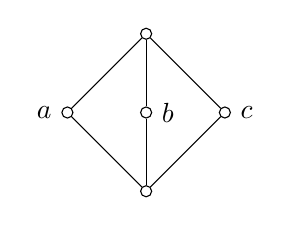
\begin{tikzpicture}
[dot/.style={circle,draw,minimum width=4pt,inner sep=1pt}]
\node[dot,label=left:$a$] (a) at (0,0) {};
\node[dot,label=right:$b$] (b) at (1,0) {};
\node[dot,label=right:$c$] (c) at (2,0) {};
\node[dot] (d) at (1,-1) {};
\node[dot] (e) at (1,1) {};
\path[] (e) edge (a) edge (b) edge (c)
(d) edge (a) edge (b) edge (c);
\end{tikzpicture}
\caption{$M_5$}
\end{subfigure}
\begin{subfigure}

\caption{$N_5$}
\end{subfigure}
\end{figure}

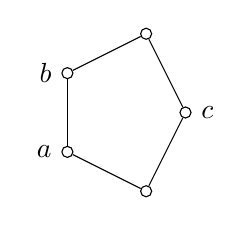
\begin{tikzpicture}
[dot/.style={circle,draw,minimum width=4pt,inner sep=1pt}]
\node[dot,label=left:$a$] (a) at (0,-0.5) {};
\node[dot,label=left:$b$] (b) at (0,0.5) {};
\node[dot,label=right:$c$] (c) at (1.5,0) {};
\node[dot] (d) at (1,1) {};
\node[dot] (e) at (1,-1) {};
\path (d) edge (b) edge (c)
(b) edge (a) 
(e) edge (a) edge (c);
\end{tikzpicture}
\end{document}
\end{document}